%%%%%%%%%%%%%%%%%%%%%%%%%%%%%%%%%%%%%%%%%%%%%%%%%%%%%%%%%%%%%%%
%PANDOC SPECIFIC SHIT, TAKEN FROM ANOTHER TEMPLATE...

\documentclass[11pt,]{article}

%Deal with margins and other geometry stuff
\usepackage[margin = 1in]{geometry}
\usepackage{longtable}
\usepackage{booktabs}

% Need to include this for refs with Pandoc

%Some of this is math package stuff, but honestly i don't really get
%what most of it is doing
\usepackage{amssymb,amsmath}
\usepackage{ifxetex,ifluatex}
\usepackage{fixltx2e} % provides \textsubscript

%Numbered section spacing
\setcounter{secnumdepth}{0}

\usepackage{setspace}
\setstretch{1}

%For LIST (enumerate) spacing
\providecommand{\tightlist}{%
  \setlength{\itemsep}{0pt}\setlength{\parskip}{0pt}}

%%%%%%%%%%%%%%%%%%%%%%%%%%%%%%%%%%%%%%%%%%%%%%%%%%%%%%%%%%%%%%%%%%%
%% LUCY'S DOCUMENT PREAMBLE AND PACKAGES

\usepackage{pdflscape}
\usepackage{xcolor}

\usepackage{tcolorbox}
\newtcolorbox{blackbox}{
  colback=white,
  colframe=black,
  coltext=black,
  boxsep=5pt,
  arc=4pt}

%\usepackage[round]{natbib}
\usepackage[sectionbib, natbibapa]{apacite} 
\usepackage[hyphens]{url}

%Set paragraph indent and between paragraph spacing
\usepackage{parskip}
\setlength\parindent{0pt}
\setlength{\parskip}{0pt}

%Need all these for graphics and tables
\usepackage{subfig}
\usepackage{graphicx}
\usepackage{blindtext}
\usepackage{array}
\usepackage{float}

%Deal with titles and make them less stupid and ugly
\usepackage{titlesec}
\titleformat{\section}[block]{\bfseries\sc\filcenter}{}{1em}{}
%\titleformat{\section}[block]{\Large\bfseries\filcenter}{}{1em}{}
\titleformat{\subsection}[hang]{\bfseries}{}{1em}{}
\setcounter{secnumdepth}{0}

\usepackage[hyphens]{url}

%Bunch of hyperlink shit
\usepackage{hyperref}
\hypersetup{
    colorlinks=true,
    linkcolor=blue,
    filecolor=magenta,      
    urlcolor=cyan,
    citecolor = black
}


%Header and footer junk
\usepackage{fancyhdr}
\pagestyle{fancy}
\fancyhead[L,C]{}
\fancyhead[R]{\small{\textsc{L E Delaney} \hspace{3mm} \textit{Chapters
1 \& 2 Homework}}}
\fancyfoot[L]{\tiny{\textit{Version date: \today}}}
    \fancyfoot[R]{\thepage}
\fancyfoot[C]{}


%%%%%%%%%%%%%%%%%%%%%%%%%%%%%%%%%%%%%%%%%%%%%%%%%%%%%%%%%%%%%%%%%%%%%%%
%% START OF THE DOCUMENT BODY
\begin{document}

%%%%%% TITLE 
\begin{center}
\Large{\textsc{Chapters 1 \& 2 Homework}}\\ \small{\textit{Ordered by
topic: DNA structure \& function; mitosis \& meiosis; inheritance
patterns; monohybrid crosses; pedigrees}}\\
\vspace*{\baselineskip}
\end{center}

%%%%%%%%%%%%%% DOCUMENT BODY
\begin{blackbox}
5. Consider Figure 1-8a. \begin{enumerate} 
 \item[a.]{ What do the small blue spheres represent? } 
 \item[b.]{ What do the brown slabs represent? } 
 \item[c.]{ Do you agree with the analogy that DNA is structured like a ladder? } 
 \end{enumerate}

\


\begin{center}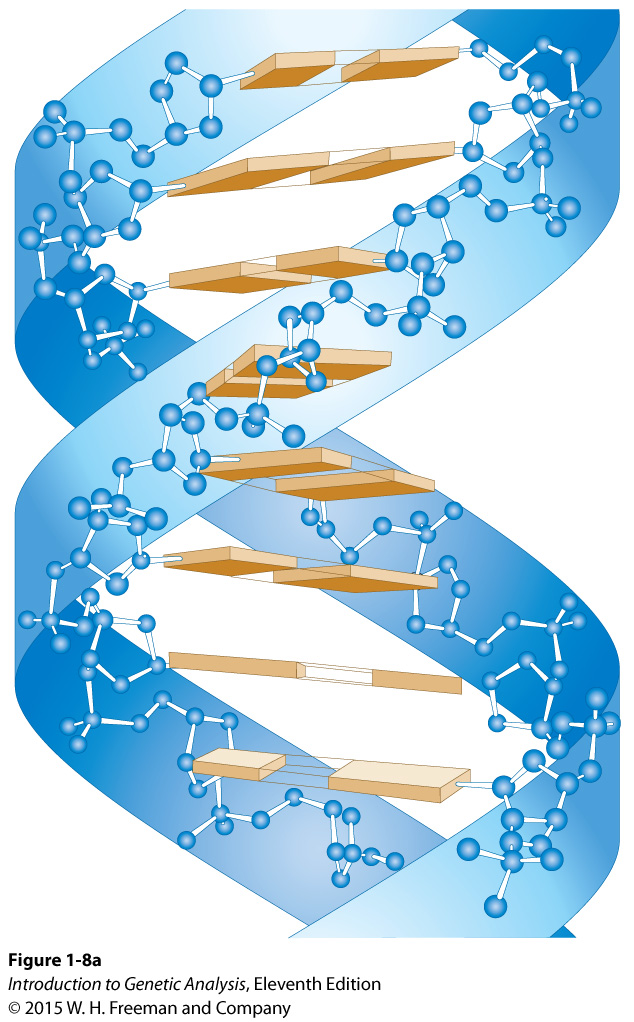
\includegraphics[width=0.25\linewidth,]{input/figure_01_08a} \end{center}


\vspace{11cm}

\end{blackbox}

\begin{blackbox}

\begin{enumerate}
\def\labelenumi{\arabic{enumi}.}
\setcounter{enumi}{5}
\tightlist
\item
  In Figure 1-8b, can you tell if the number of hydrogen bonds between
  adenine and thymine is the same as that between cytosine and guanine?
  Do you think that a DNA molecule with a high content of A + T would be
  more stable than one with a high content of G + C?
\end{enumerate}

\hfill\break

\begin{center}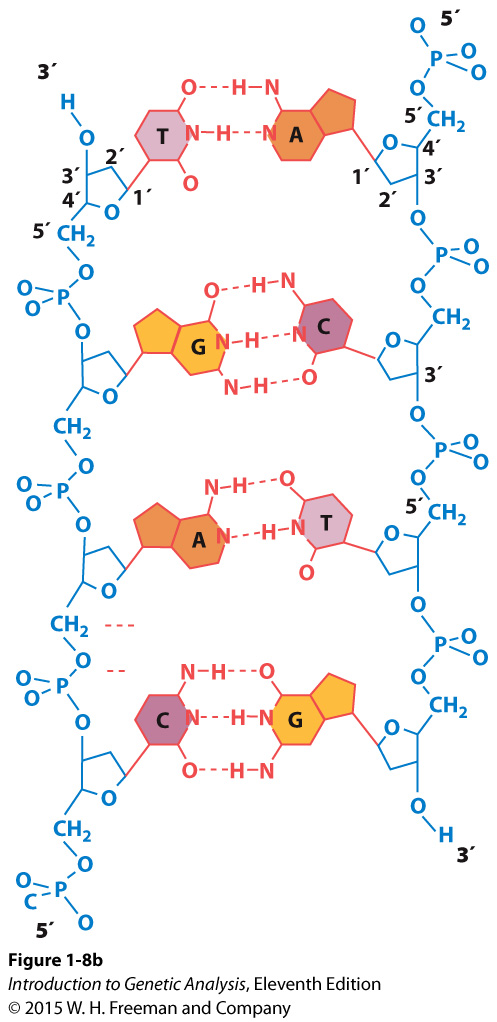
\includegraphics[width=0.25\linewidth,]{input/figure_01_08b} \end{center}

\vspace{11cm}

\end{blackbox}

\begin{blackbox}

\begin{enumerate}
\def\labelenumi{\arabic{enumi}.}
\setcounter{enumi}{9}
\tightlist
\item
  Below is the sequence of a single strand of a short DNA molecule. On a
  piece of paper, rewrite this sequence and then write the sequence of
  the complementary strand below it.
\end{enumerate}

\vspace{10mm}

\begin{center}

GTTCGCGGCCGCGAAC

\vspace{10mm}
\end{center}

Comparing the top and bottom strands, what do you notice about the
relationship between them?

\vspace{17cm}

\end{blackbox}

\begin{blackbox}

\begin{enumerate}
\def\labelenumi{\arabic{enumi}.}
\setcounter{enumi}{11}
\tightlist
\item
  If a DNA double helix that is 100 base pairs in length has 32
  adenines, how many cytosines, guanines, and thymines must it have?
\end{enumerate}

\vspace{19cm}

\end{blackbox}

\begin{landscape}

\begin{center}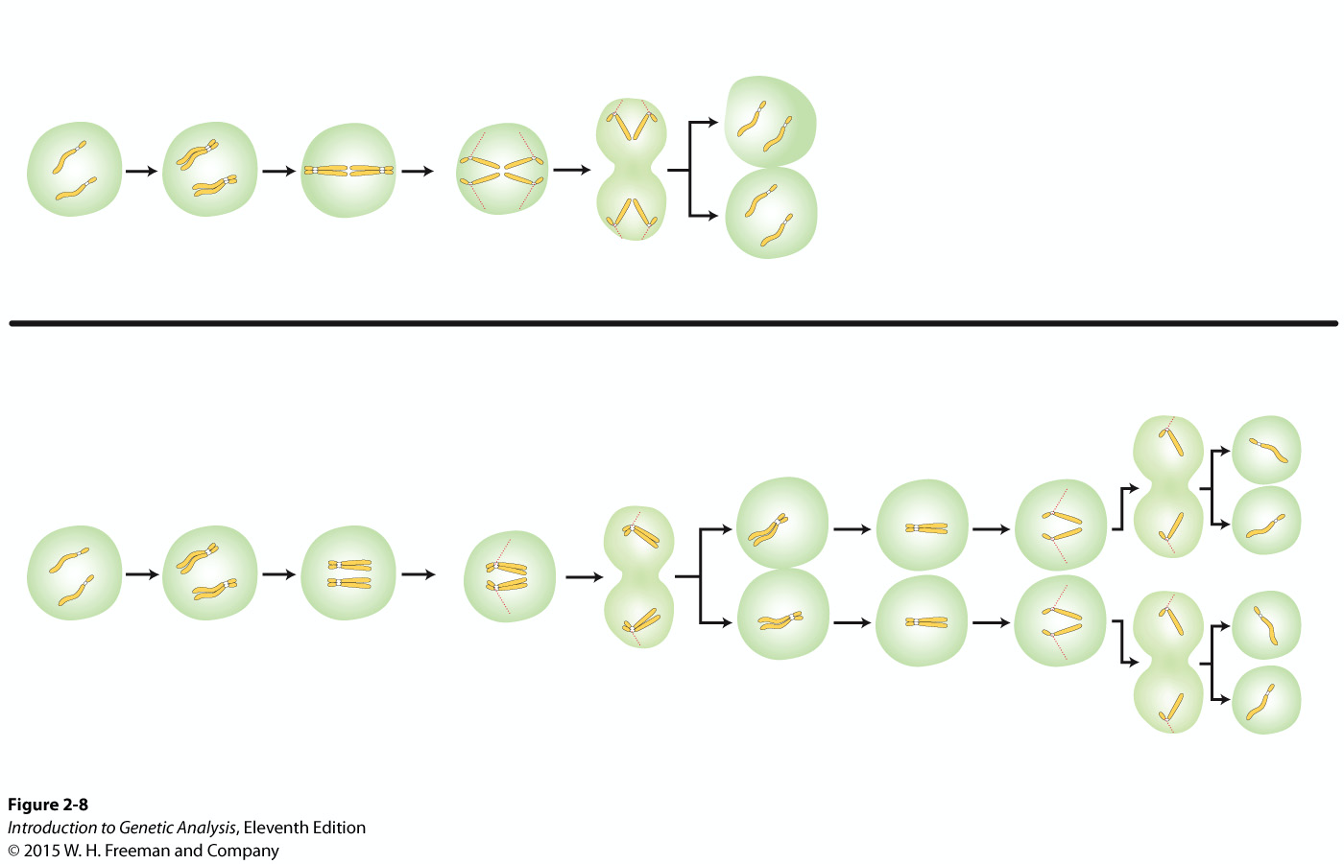
\includegraphics[width=1\linewidth,]{input/mitosis-meiosis} \end{center}

\end{landscape}

\begin{blackbox}

\begin{enumerate}
\def\labelenumi{\arabic{enumi}.}
\setcounter{enumi}{17}
\tightlist
\item
  Name the key function of mitosis.
\end{enumerate}

\vspace{19cm}

\end{blackbox}

\begin{blackbox}

\begin{enumerate}
\def\labelenumi{\arabic{enumi}.}
\setcounter{enumi}{18}
\tightlist
\item
  Name two key functions of meiosis.
\end{enumerate}

\vspace{19cm}

\end{blackbox}

\begin{blackbox}

\begin{enumerate}
\def\labelenumi{\arabic{enumi}.}
\setcounter{enumi}{21}
\tightlist
\item
  In what ways does the second division of meiosis differ from mitosis?
\end{enumerate}

\vspace{19cm}

\end{blackbox}

\begin{blackbox}

\begin{enumerate}
\def\labelenumi{\arabic{enumi}.}
\setcounter{enumi}{29}
\tightlist
\item
  Four of the following events are part of both meiosis and mitosis, but
  only one is meiotic. Which one? (1) chromatid formation, (2) spindle
  formation, (3) chromosome condensation, (4) chromo- some movement to
  poles, (5) synapsis
\end{enumerate}

\vspace{19cm}

\end{blackbox}

\begin{landscape}

\begin{center}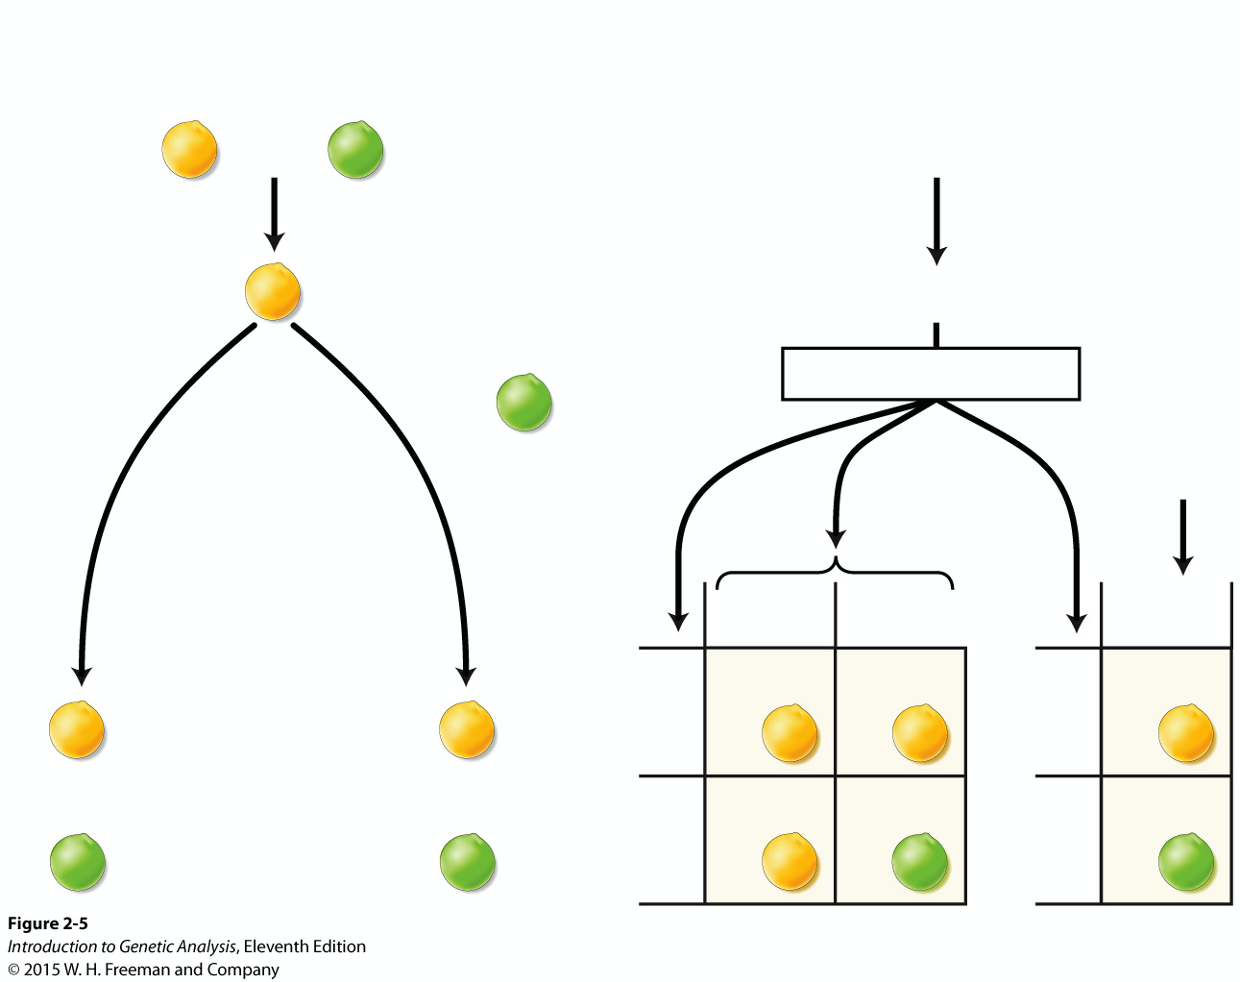
\includegraphics[width=0.9\linewidth,]{input/mendel-ratio} \end{center}

\end{landscape}

\begin{blackbox}

11. Mendel studied a tall variety of pea plants with stems that are 20 cm long and a dwarf variety with stems that are only 12 cm long. \begin{enumerate} 
 \item[a.]{ Under blending theory, how long would you expect the stems of first and second hybrids to be? } 
 \item[b.]{ Under Mendelian rules, what would you expect to observe in the second-generation hybrids if all the first-generation hybrids were tall? } 
 \end{enumerate}

\vspace{19cm}


\end{blackbox}

\begin{blackbox}

\begin{enumerate}
\def\labelenumi{\arabic{enumi}.}
\setcounter{enumi}{45}
\tightlist
\item
  Suppose that a husband and wife are both heterozygous for a recessive
  allele for albinism. If they have dizygotic (two-egg) twins, what is
  the probability that both the twins will have the same phenotype for
  pigmentation?
\end{enumerate}

\vspace{20cm}

\end{blackbox}

\begin{blackbox}

\begin{enumerate}
\def\labelenumi{\arabic{enumi}.}
\setcounter{enumi}{26}
\tightlist
\item
  If children obtain half their genes from one parent and half from the
  other parent, why aren't siblings identical?
\end{enumerate}

\vspace{19cm}

\end{blackbox}

\begin{blackbox}

\begin{enumerate}
\def\labelenumi{\arabic{enumi}.}
\setcounter{enumi}{3}
\tightlist
\item
  Figure 1-7 shows a simplified pathway for arginine synthesis in
  Neurospora. Suppose you have a special strain of Neurospora that makes
  citrulline but not arginine. Which gene(s) are likely mutant or
  missing in your special strain? You have a second strain of Neurospora
  that makes neither citrulline nor arginine but does make ornithine.
  Which gene(s) are mutant or missing in this strain?\\
\end{enumerate}

\begin{center}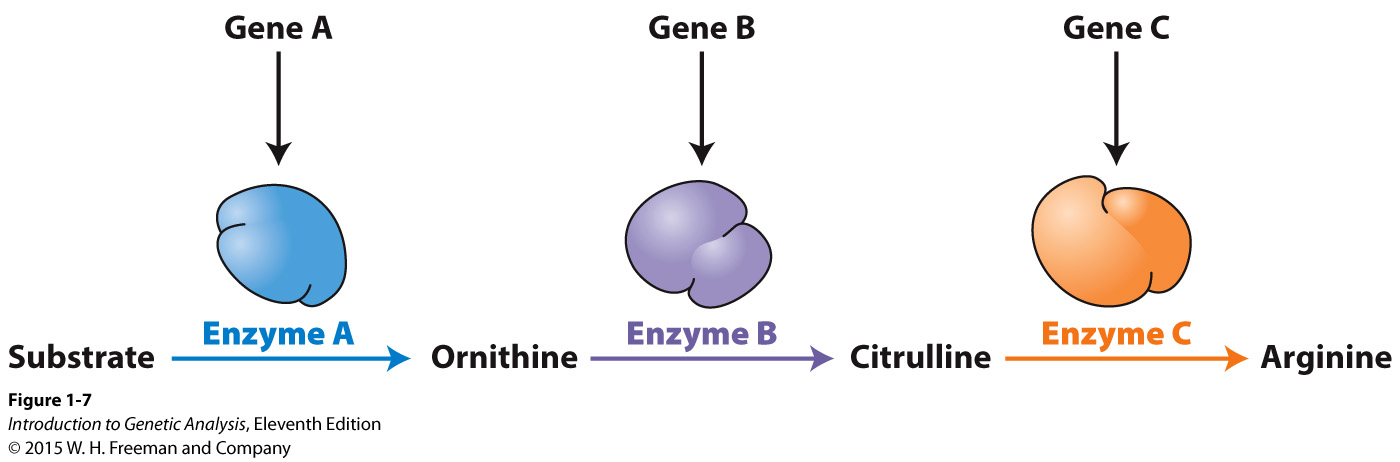
\includegraphics[width=0.45\linewidth,]{input/figure_01_07} \end{center}

\vspace{17cm}

\end{blackbox}

\begin{blackbox}

\begin{enumerate}
\def\labelenumi{\arabic{enumi}.}
\tightlist
\item
  If the white-flowered parental variety in Figure 1-3 were crossed to
  the first-generation hybrid plant in that figure, what types of
  progeny would you expect to see and in what proportions?
\end{enumerate}

\begin{center}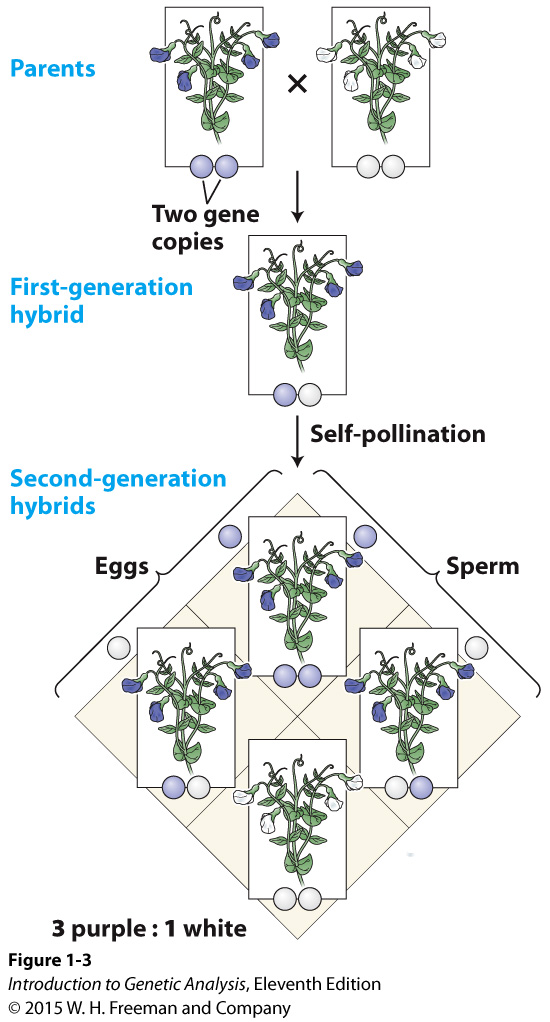
\includegraphics[width=0.35\linewidth,]{input/figure_01_03} \end{center}

\vspace{9cm}

\end{blackbox}

\begin{blackbox}

\begin{enumerate}
\def\labelenumi{\arabic{enumi}.}
\setcounter{enumi}{1}
\tightlist
\item
  In the right-hand part of Figure 2-4, in the plant showing an 11:11
  ratio, do you think it would be possible to find a pod with all yellow
  peas? All green? Explain.
\end{enumerate}

\hfill\break

\begin{center}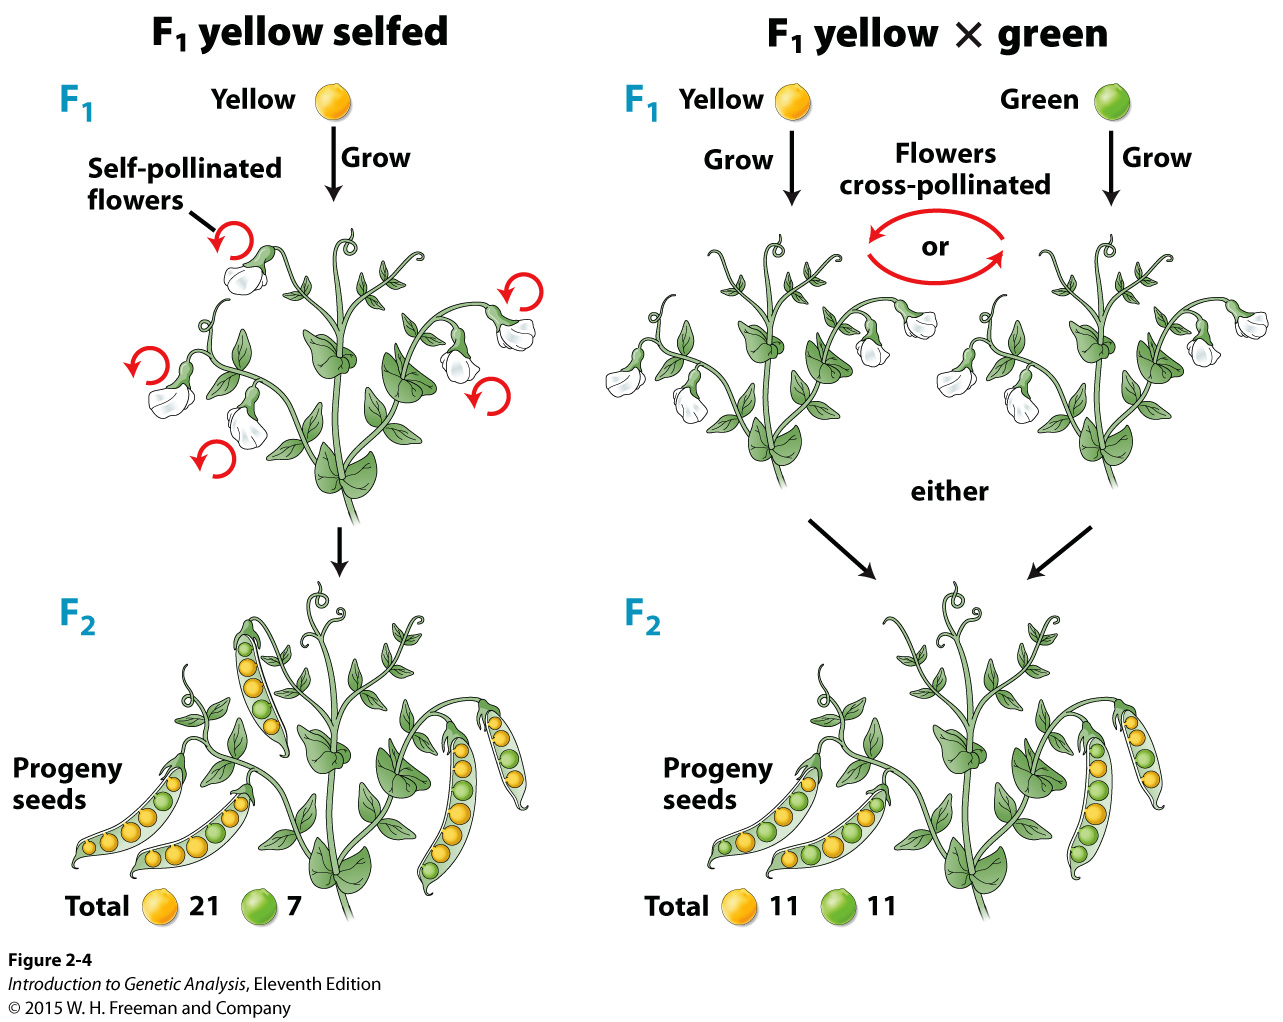
\includegraphics[width=0.65\linewidth,]{input/figure_02_04} \end{center}

\vspace{12cm}

\end{blackbox}

\begin{blackbox}

\begin{enumerate}
\def\labelenumi{\arabic{enumi}.}
\setcounter{enumi}{2}
\tightlist
\item
  In Table 2-1, state the recessive phenotype in each of the seven
  cases.
\end{enumerate}

\hfill\break

\begin{center}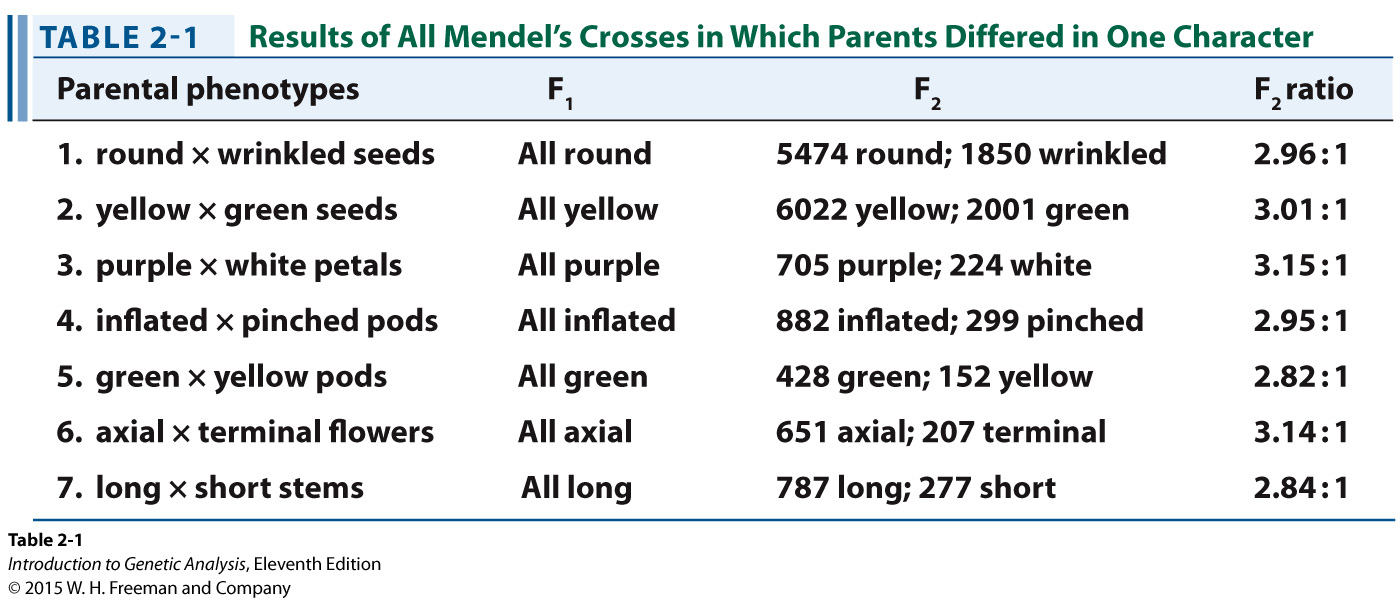
\includegraphics[width=0.65\linewidth,]{input/table_02_01} \end{center}

\vspace{14cm}

\end{blackbox}

\begin{blackbox}

\begin{enumerate}
\def\labelenumi{\arabic{enumi}.}
\setcounter{enumi}{39}
\tightlist
\item
  In the plant \emph{Arabidopsis thaliana}, a geneticist is interested
  in the development of trichomes (small projections). A large screen
  turns up two mutant plants (A and B) that have no trichomes, and these
  mutants seem to be potentially useful in studying trichome
  development. (If they were determined by single-gene mutations, then
  finding the normal and abnormal functions of these genes would be
  instructive.) Each plant is crossed with wild type; in both cases, the
  next generation (F1) had normal trichomes. When F1 plants were selfed,
  the resulting F2's were as follows:
\end{enumerate}

\vspace{8mm}

\begin{itemize}
\tightlist
\item
  F2 from mutant A: 602 normal; 198 no trichomes
\item
  F2 from mutant B: 267 normal; 93 no trichomes
\end{itemize}

\vspace{8mm}

\begin{enumerate} 
 \item[a.]{ What do these results show? Include proposed genotypes of all plants in your answer. } 
 \item[b.]{ Under your explanation to part a, is it possible to confidently predict the F1 from crossing the original mutant A with the original mutant B?  } 
 \end{enumerate}

\vspace{12cm}

\end{blackbox}

\begin{blackbox}

\begin{enumerate}
\def\labelenumi{\arabic{enumi}.}
\setcounter{enumi}{48}
\tightlist
\item
  In nature, the plant \emph{Plectritis congesta} is dimorphic for fruit
  shape; that is, individual plants bear either wingless or winged
  fruits. Plants were collected from nature before flowering and were
  crossed or selfed with the following results:
\end{enumerate}

\hfill\break

\begin{longtable}[]{@{}lll@{}}
\toprule
Pollination & Winged & Wingless\tabularnewline
\midrule
\endhead
Winged (selfed) & 91 & 1\tabularnewline
Winged (selfed) & 90 & 30\tabularnewline
Wingless (selfed) & 4 & 80\tabularnewline
Winged x wingless & 161 & 0\tabularnewline
Winged x wingless & 29 & 31\tabularnewline
Winged x wingless & 46 & 0\tabularnewline
Winged x winged & 44 & 0\tabularnewline
Winged x winged & 24 & 0\tabularnewline
\bottomrule
\end{longtable}

\begin{center}\rule{0.5\linewidth}{0.5pt}\end{center}

\hfill\break

\begin{longtable}[]{@{}llll@{}}
\toprule
Pollination & Genotypes & Winged & Wingless\tabularnewline
\midrule
\endhead
Winged (selfed) & & 91 & 1\tabularnewline
Winged (selfed) & & 90 & 30\tabularnewline
Wingless (selfed) & & 4 & 80\tabularnewline
Winged x wingless & & 161 & 0\tabularnewline
Winged x wingless & & 29 & 31\tabularnewline
Winged x wingless & & 46 & 0\tabularnewline
Winged x winged & & 44 & 0\tabularnewline
Winged x winged & & 24 & 0\tabularnewline
\bottomrule
\end{longtable}

\vspace{7cm}

\end{blackbox}

\begin{blackbox}

\begin{enumerate}
\def\labelenumi{\arabic{enumi}.}
\setcounter{enumi}{41}
\item
  \begin{enumerate} 
   \item[a.]{ The ability to taste the chemical phenylthiocarbamide is an autosomal dominant phenotype, and the inability to taste it is recessive. If a taster woman with a nontaster father marries a taster man who had a nontaster daughter in a previous marriage, what is the probability that their first child will be: (1) a nontaster girl, (2) a taster girl, or (3) a taster boy? } 
   \item[b.]{ What is the probability that their first two children will be tasters of either sex? } 
   \end{enumerate}
\end{enumerate}

\hfill\break

\vspace{17cm}

\end{blackbox}

\begin{blackbox}

\begin{enumerate}
\def\labelenumi{\arabic{enumi}.}
\setcounter{enumi}{42}
\tightlist
\item
  In the pedigree below, the black symbols represent individuals with a
  very rare blood disease. If you had no other information to go on,
  would you think it more likely that the disease was dominant or
  recessive? Give your reasons.
\end{enumerate}

\hfill\break

\begin{center}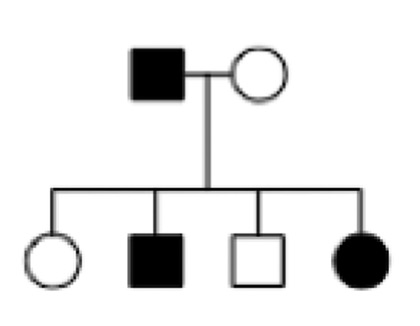
\includegraphics[width=0.35\linewidth,]{input/43pedigree} \end{center}

\vspace{15cm}

\end{blackbox}

\begin{blackbox}

\begin{enumerate}
\def\labelenumi{\arabic{enumi}.}
\setcounter{enumi}{12}
\tightlist
\item
  Could the pedigree in Figure 2-31 be explained as an autosomal
  dominant disorder? Explain.
\end{enumerate}

\hfill\break

\begin{center}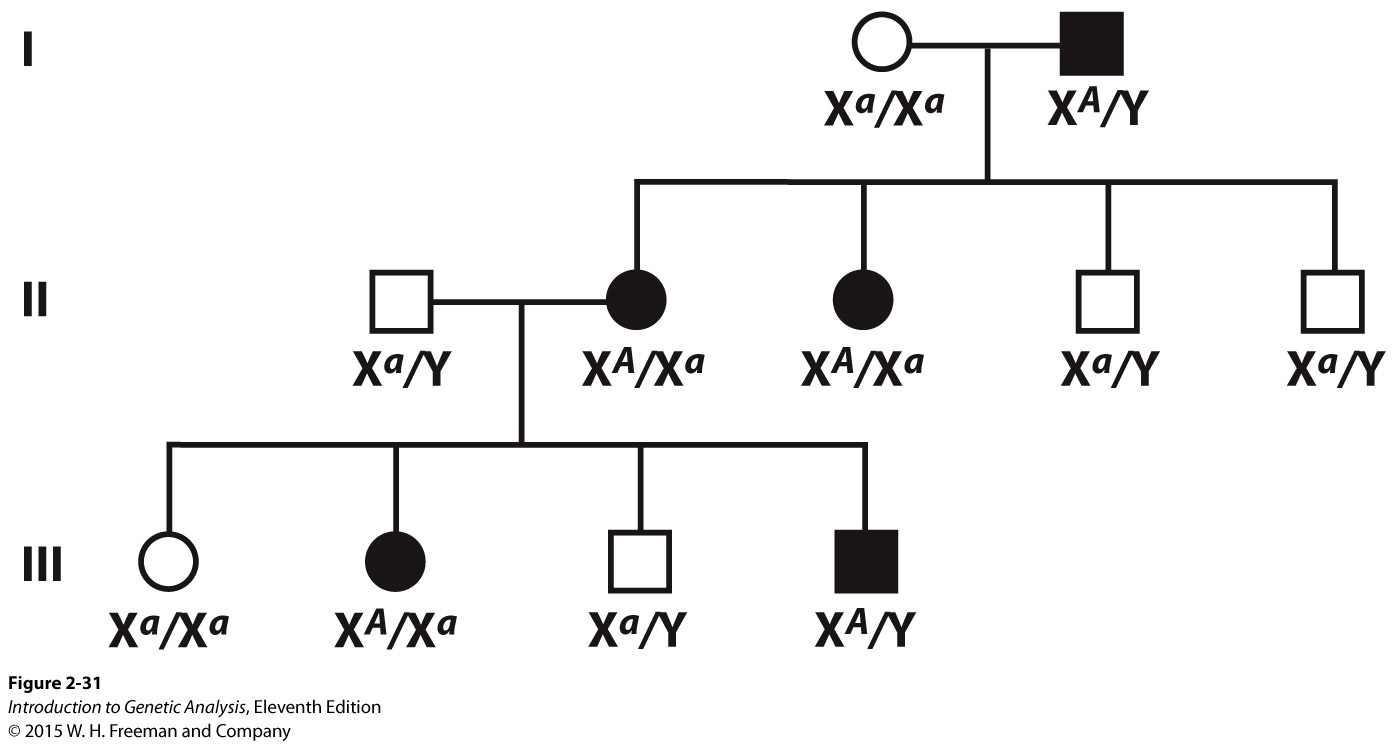
\includegraphics[width=0.55\linewidth,]{input/figure_02_31} \end{center}

\vspace{14cm}

\end{blackbox}

\begin{blackbox}

\begin{enumerate}
\def\labelenumi{\arabic{enumi}.}
\setcounter{enumi}{49}
\tightlist
\item
  The accompanying pedigree is for a rare but relatively mild hereditary
  disorder of the skin.

  \begin{enumerate} 
   \item[a.]{ How is the disorder inherited? State reasons for your answer. } 
   \item[b.]{ Give genotypes for as many individuals in the pedigree as possible. (Invent your own defined allele symbols.) } 
   \item[c.]{ Consider the four unaffected children of parents III-4 and III-5. In all four-child progenies from parents of these genotypes, what proportion is expected to contain all unaffected children? } 
   \end{enumerate}
\end{enumerate}

\hfill\break

\begin{center}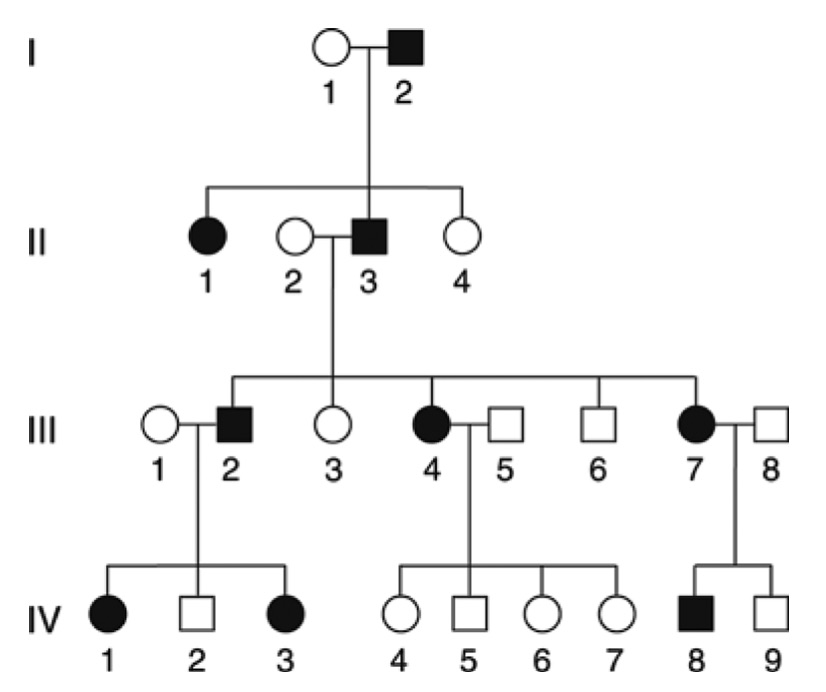
\includegraphics[width=0.55\linewidth,]{input/50pedigree} \end{center}

\vspace{9cm}

\end{blackbox}

\begin{blackbox}

\begin{enumerate}
\def\labelenumi{\arabic{enumi}.}
\setcounter{enumi}{52}
\tightlist
\item
  The following pedigree was obtained for a rare kidney disease.

  \begin{enumerate} 
   \item[a.]{ Deduce the inheritance of this condition, stating your reasons. } 
   \item[b.]{ If persons 1 and 2 marry, what is the probability that their first child will have the kidney disease? } 
   \end{enumerate}
\end{enumerate}

\hfill\break

\begin{center}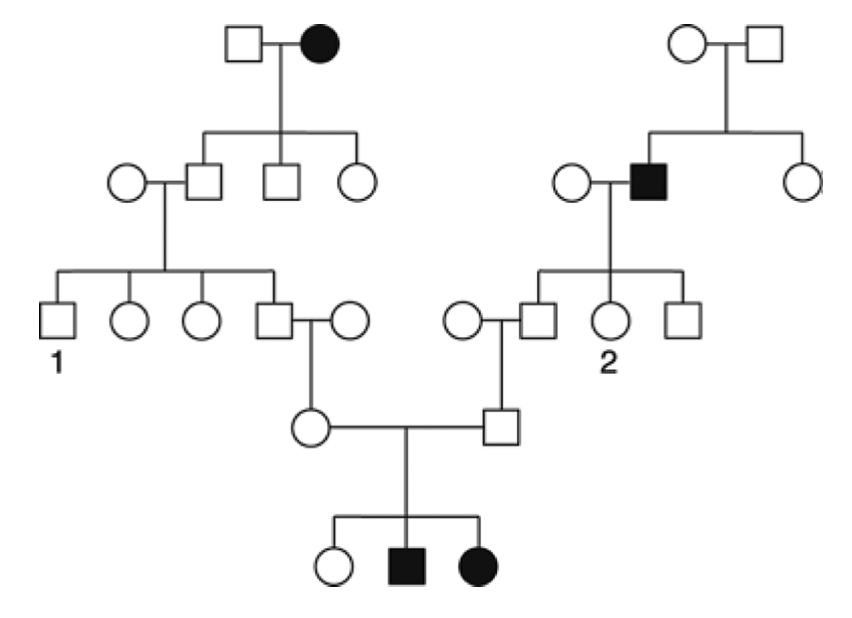
\includegraphics[width=0.55\linewidth,]{input/53pedigree} \end{center}

\vspace{12cm}

\end{blackbox}

\begin{blackbox}

\begin{enumerate}
\def\labelenumi{\arabic{enumi}.}
\setcounter{enumi}{60}
\tightlist
\item
  Duchenne muscular dystrophy is sex-linked and usually affects only
  males. Victims of the disease become progressively weaker, starting
  early in life.

  \begin{enumerate} 
   \item[a.]{ What is the probability that a woman whose brother has Duchenne’s disease will have an affected child? } 
   \item[b.]{ If your mother’s brother (your uncle) had Duchenne’s disease, what is the probability that you have received the allele? } 
   \item[c.]{ If your father’s brother had the disease, what is the probability that you have received the allele? } 
   \end{enumerate}
\end{enumerate}

\hfill\break

\vspace{17cm}

\end{blackbox}

\end{document}


